\documentclass[a4paper,11pt,singlespacing]{article}

\usepackage{setspace}
\usepackage[utf8]{inputenc}
\usepackage[T1]{fontenc}
\usepackage{graphicx}
\usepackage{color}
\usepackage{hyperref}
\usepackage{listings,xcolor}
\usepackage{pdfpages}

\renewcommand{\figurename}{Abbildung}

\graphicspath{ {./images/} }



\begin{document}
	\setlength{\parindent}{0ex}
	
	\begin{titlepage}
		\author{Luca Asmus\\ Marius Würstle\\Rolf Wiersch}
		\title{
\includegraphics[scale=0.3]{rwu_logo_hor-lila-cyan_rgb_0} \\ ~\\ ~\\ WLAN-AP mit regelmäßigem PSK-Tausch und QR-Code Anmeldung \vspace{8cm}}
		\date{\today}
		\maketitle
		\thispagestyle{empty}
    	\end{titlepage}
    	
    	\section{Zusammenfassung}
    	\tableofcontents
    	
    	\section{Abbildungsverzeichnis}
    	\listoffigures
    	\newpage
    	
    	\section{Allgemeines}
    	
    	\section{Fachbegriffe}
    	
    	\section{Hardware}
    		\subsection{Raspberry Pi}
    			Der Raspberry Pi ist wurde für junge Menschen entwickelt, um ihnen eine preisgünstige Möglichkeit zu bieten, sich mit der Informatik zu beschäftigen. Der Einplatinencomputer ist etwa Kreditkartengroß und kam Anfang 2012 auf den Markt. Er ermöglicht einen schnellen und praktischen Weg um Wissen in den Bereichen Programmieren und Hardware. Zudem ist er vielseitig einsetzbar in diesem Fall wird er zu einem Access-Point konfiguriert. 
    			\begin{figure}[ht]
    				\centering
	    			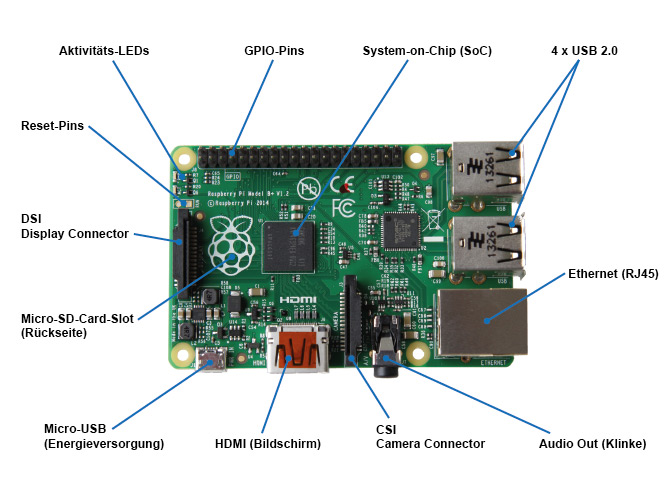
\includegraphics[scale=0.5]{raspberry_pi_3b}
	    				\caption{Raspberry Pi 3b}
	    				\label{raspberrypi3b}
			\end{figure}
			Technische Spezifikationen unseres Raspberry Pi 3b:
			\begin{itemize}
				\item Quad Core 1.2GHz Broadcom BCM2837 64bit CPU
				\item 1GB RAM
				\item BCM43438 wireless LAN and Bluetooth Low Energy (BLE) on board
				\item 100 Base Ethernet
				\item 40-pin extended GPIO
				\item 4 USB 2 ports
				\item 4 Pole stereo output and composite video port
				\item Full size HDMI
				\item CSI camera port for connecting a Raspberry Pi camera
				\item DSI display port for connecting a Raspberry Pi touchscreen display
				\item Micro SD port for loading your operating system and storing data
				\item Upgraded switched Micro USB power source up to 2.5A
			\end{itemize}
		\subsection{RASP PI 3.2 in TD}
			image + Buttons und touchscreen
		\subsection{SD-Karte}
    			32GB
    			
    	\section{Software}
    		\subsection{balenaEtcher}
    			Flash Sd Card
		\subsection{hostapd}
    		\subsection{dnsmasq}
    		\subsection{cron}
			Planen der Ausführung des Skripts
    		\subsection{Python3.7}
    			\subsubsection{pyqrcode}
    			\subsubsection{gpiozero}
    	\section{Konfiguration des Raspberry Pi als Access-Point}
    	
    	\section{Passwortgenerierung}
    	
    	\section{Ausgabe des Passworts}
    	
    	\section{Fazit mit Ausblick}
    	
    	\section{Quellenverzeichnis}
    	
    	\url{http://www.elektronik-kompendium.de/sites/raspberry-pi/bilder/19052512.jpg} [aufgerufen am 25.11.2020] \ref{raspberrypi3b}
    	
\end{document}
